\documentclass[11  pt]{article} 
\usepackage[lmargin=1in,rmargin=1.75in,bmargin=1in,tmargin=1in]{geometry}  


% For hyperlinking everything
\usepackage{hyperref}
\hypersetup{
	colorlinks=true, %set true if you want colored links
	linktoc=all,     %set to all if you want both sections and subsections linked
	linkcolor=blue,  %choose some color if you want links to stand out
}


\usepackage[latin1]{inputenc}
\usepackage{amsmath}
\usepackage{mathrsfs}  
\usepackage{amsfonts}
\usepackage{amssymb}
\usepackage{graphicx}
\usepackage{subfig}
\usepackage{caption}
\usepackage{algorithm}
%\usepackage{algcompatible}
%\usepackage{algorithmicx}
\usepackage{algpseudocode}

\usepackage{titlesec}
\titleformat{\section}{\fontfamily{lmss}\fontsize{14}{15}\bfseries}{\thesection}{1em}{}
\titleformat{\subsection}{\fontfamily{lmss}\fontsize{12}{15}\bfseries}{\thesubsection}{1em}{}




\usepackage{amsthm}

\newtheoremstyle{noit}
{10pt}% <Space above>
{10pt}% <Space below>
{}% <Body font>
{}% <Indent amount>
{\bfseries}% <Theorem head font>
{.}% <Punctuation after theorem head>
{.5em}% <Space after theorem headi>
{}% <Theorem head spec (can be left empty, meaning `normal')>

\newtheoremstyle{example}
{10pt}% <Space above>
{10pt}% <Space below>
{}% <Body font>
{20pt}% <Indent amount>
{\bfseries}% <Theorem head font>
{.}% <Punctuation after theorem head>
{.5em}% <Space after theorem headi>
{}% <Theorem head spec (can be left empty, meaning `normal')>


\newtheoremstyle{indented}{20pt}{20pt}{\addtolength{\leftskip}{2.5em}}{}{\bfseries}{.}{.5em}{}


\newtheorem{theorem}{Theorem}
\numberwithin{theorem}{section}
\newtheorem{lemma}[theorem]{Lemma}
\newtheorem{corollary}[theorem]{Corollary}
\newtheorem{observation}{Observation}
%\numberwithin{observation}{section}
%\numberwithin{definition}{section}
\newtheorem{conjecture}{Conjecture}
\newtheorem{Qu}{Question}
\newcommand{\QU}{\begin{Qu}\normalfont}

\theoremstyle{noit}
\newtheorem{fact}{Fact}
\newtheorem{definition}{Definition}

\theoremstyle{indented}
\newtheorem{example}{Example}

\theoremstyle{indented}
\newtheorem{problem}{Problem}


%\newenvironment{proof}{\noindent{\bf Proof:} \hspace*{1em}}{
%    \hspace*{\fill} $\Box$ }
%\newenvironment{proof_of}[1]{\noindent {\bf Proof of #1:}
%    \hspace*{1em} }{\hspace*{\fill} $\Box$ }
%\newenvironment{proof_claim}{\begin{quotation} \noindent}{
%    \hspace*{\fill} $\diamond$ \end{quotation}}
\newcommand{\vs}[1]{\vspace{#1}}

\newcommand{\lecture}[2]{
 \noindent
\begin{center}
	\framebox{
		\vbox{
			\hbox to 5.78in { {\bf CSCE 411: Design and Analysis of Algorithms} \hfill  }
			\vspace{2mm}
			\hbox to 5.78in { {\Large \hfill Lecture #1\hfill} }
			\vspace{2mm}
			\hbox to 5.78in { {\it Date: #2 \hfill Lecturer: Nate Veldt} }
		}
	}
\end{center}
\vspace*{4mm}
}


\newcommand{\hw}[2]{
	\noindent
	\begin{center}
		\framebox{
			\vbox{
				\hbox to 5.78in { {\bf CSCE 411: Design and Analysis of Algorithms} \hfill  }
				\vspace{2mm}
				\hbox to 5.78in { {\Large \hfill Homework #1\hfill} }
				\vspace{2mm}
				\hbox to 5.78in { {\it Due date: #2 \hfil} }
			}
		}
	\end{center}
	\vspace*{4mm}
}



\newcommand{\under}[1]{\underline{\hspace{#1}}}
\setlength{\parindent}{0em}

%\usepackage[tagged]{accessibility}

% Graph terms
\newcommand{\vol}{\textbf{vol}}
\newcommand{\cut}{\textbf{cut}}


% Matrices
\newcommand{\mA}{\textbf{A}}
\newcommand{\mB}{\textbf{B}}

% vectors
\newcommand{\ve}{\textbf{e}}
\newcommand{\vx}{\textbf{x}}


% Other
\newcommand{\calN}{\mathcal{N}}

\usepackage{mathtools}
\DeclarePairedDelimiter\ceil{\lceil}{\rceil}
\DeclarePairedDelimiter\floor{\lfloor}{\rfloor}


\newcommand*{\aitem}{ \item[{
\includegraphics[width=0.8cm,height=0.5cm]{../../Lectures/figures/A}} ]  }
\newcommand*{\bitem}{ \item[{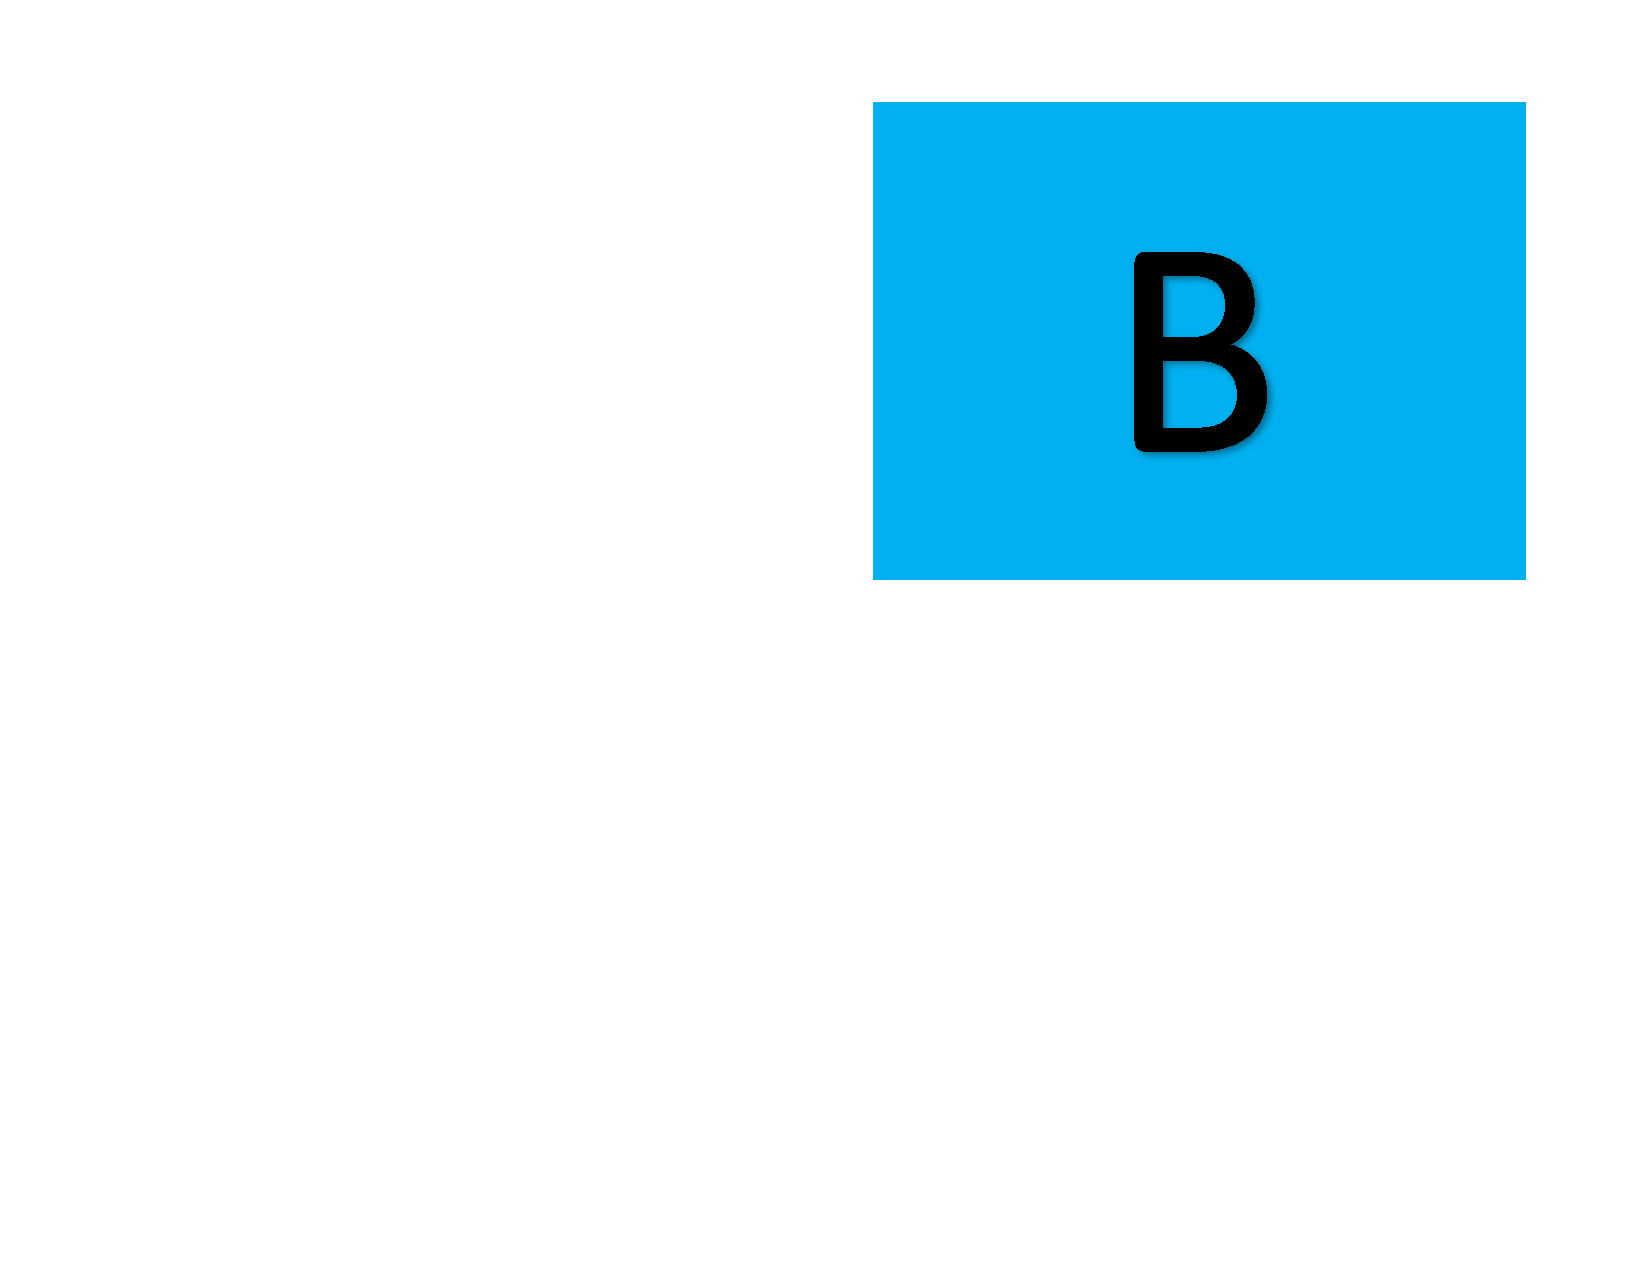
\includegraphics[width=0.8cm,height=0.5cm]{../../Lectures/figures/B}} ]  }
\newcommand*{\citem}{ \item[{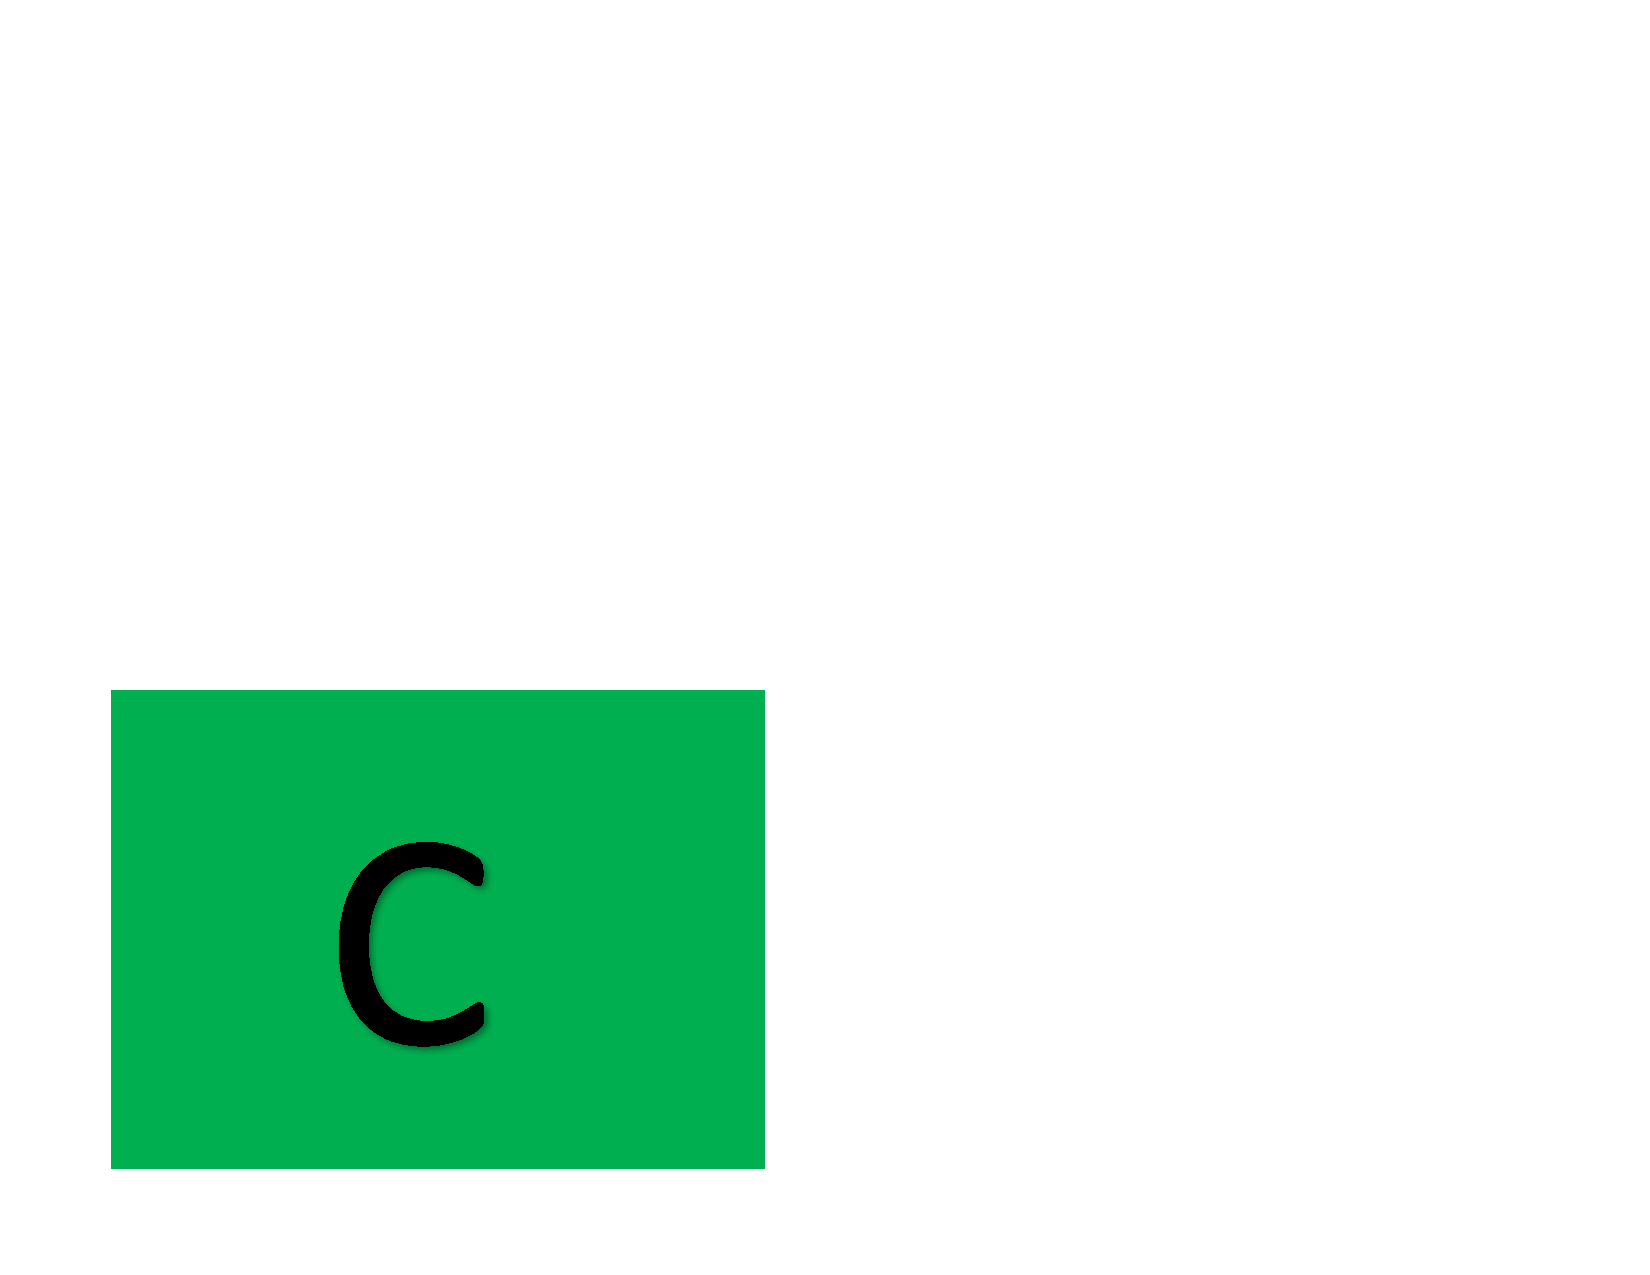
\includegraphics[width=0.8cm,height=0.5cm]{../../Lectures/figures/C}} ]  }
\newcommand*{\ditem}{ \item[{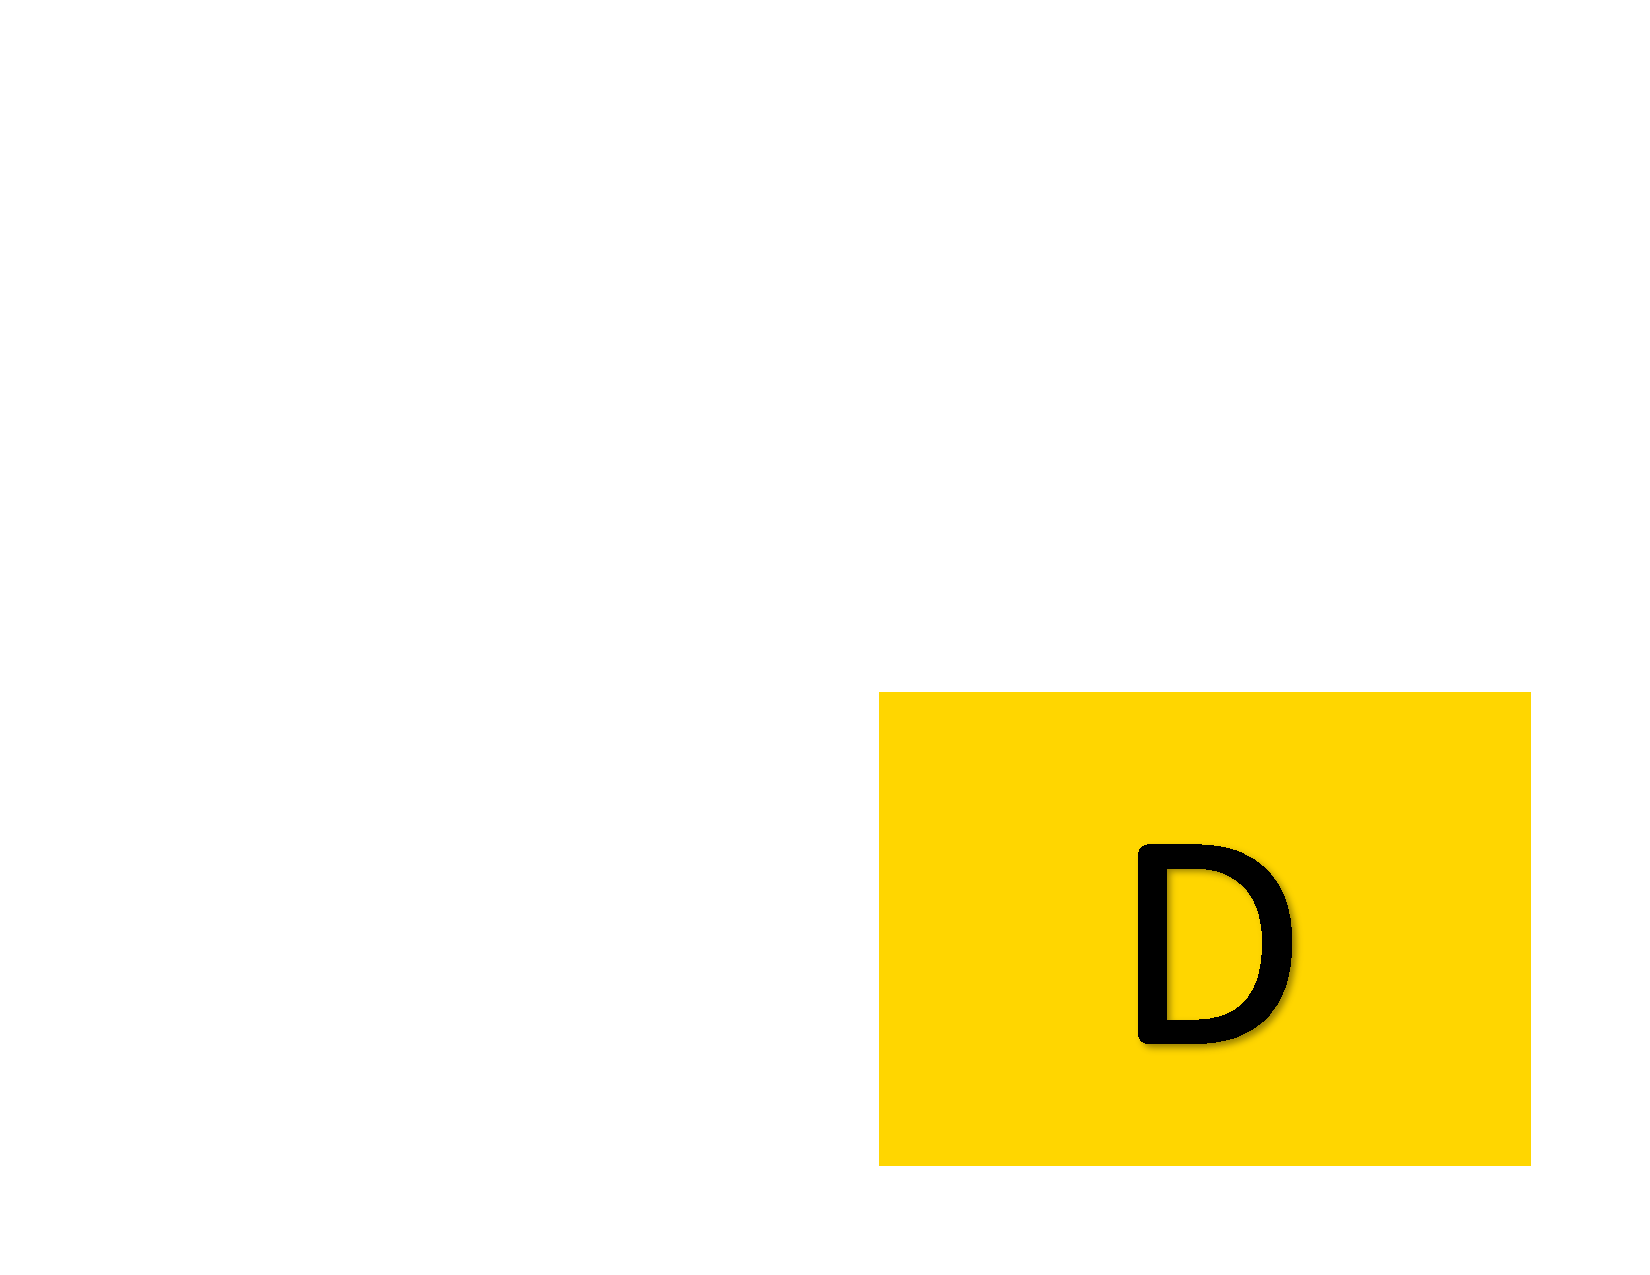
\includegraphics[width=0.8cm,height=0.5cm]{../../Lectures/figures/D}} ]  }
\newcommand*{\eitem}{ \item[{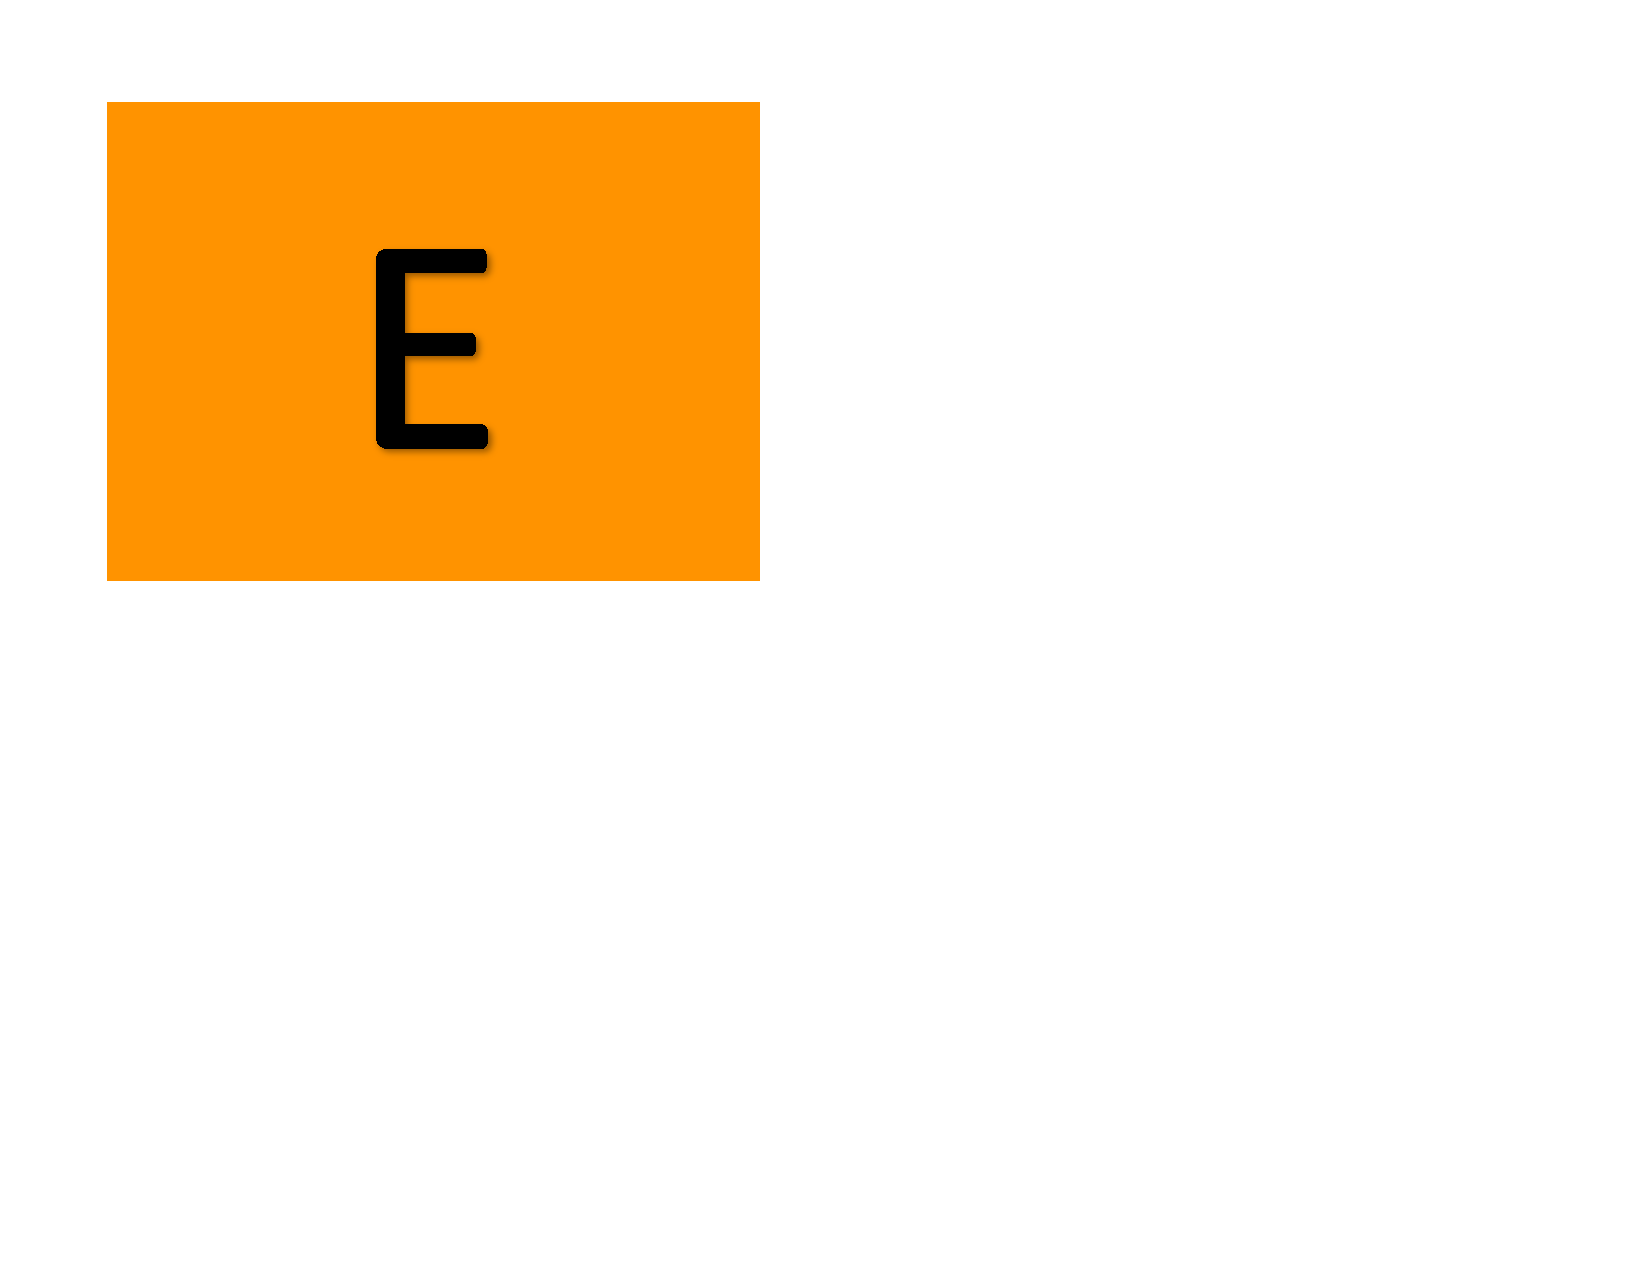
\includegraphics[width=0.8cm,height=0.5cm]{../../Lectures/figures/E}} ]  }
\newcommand*{\fitem}{ \item[{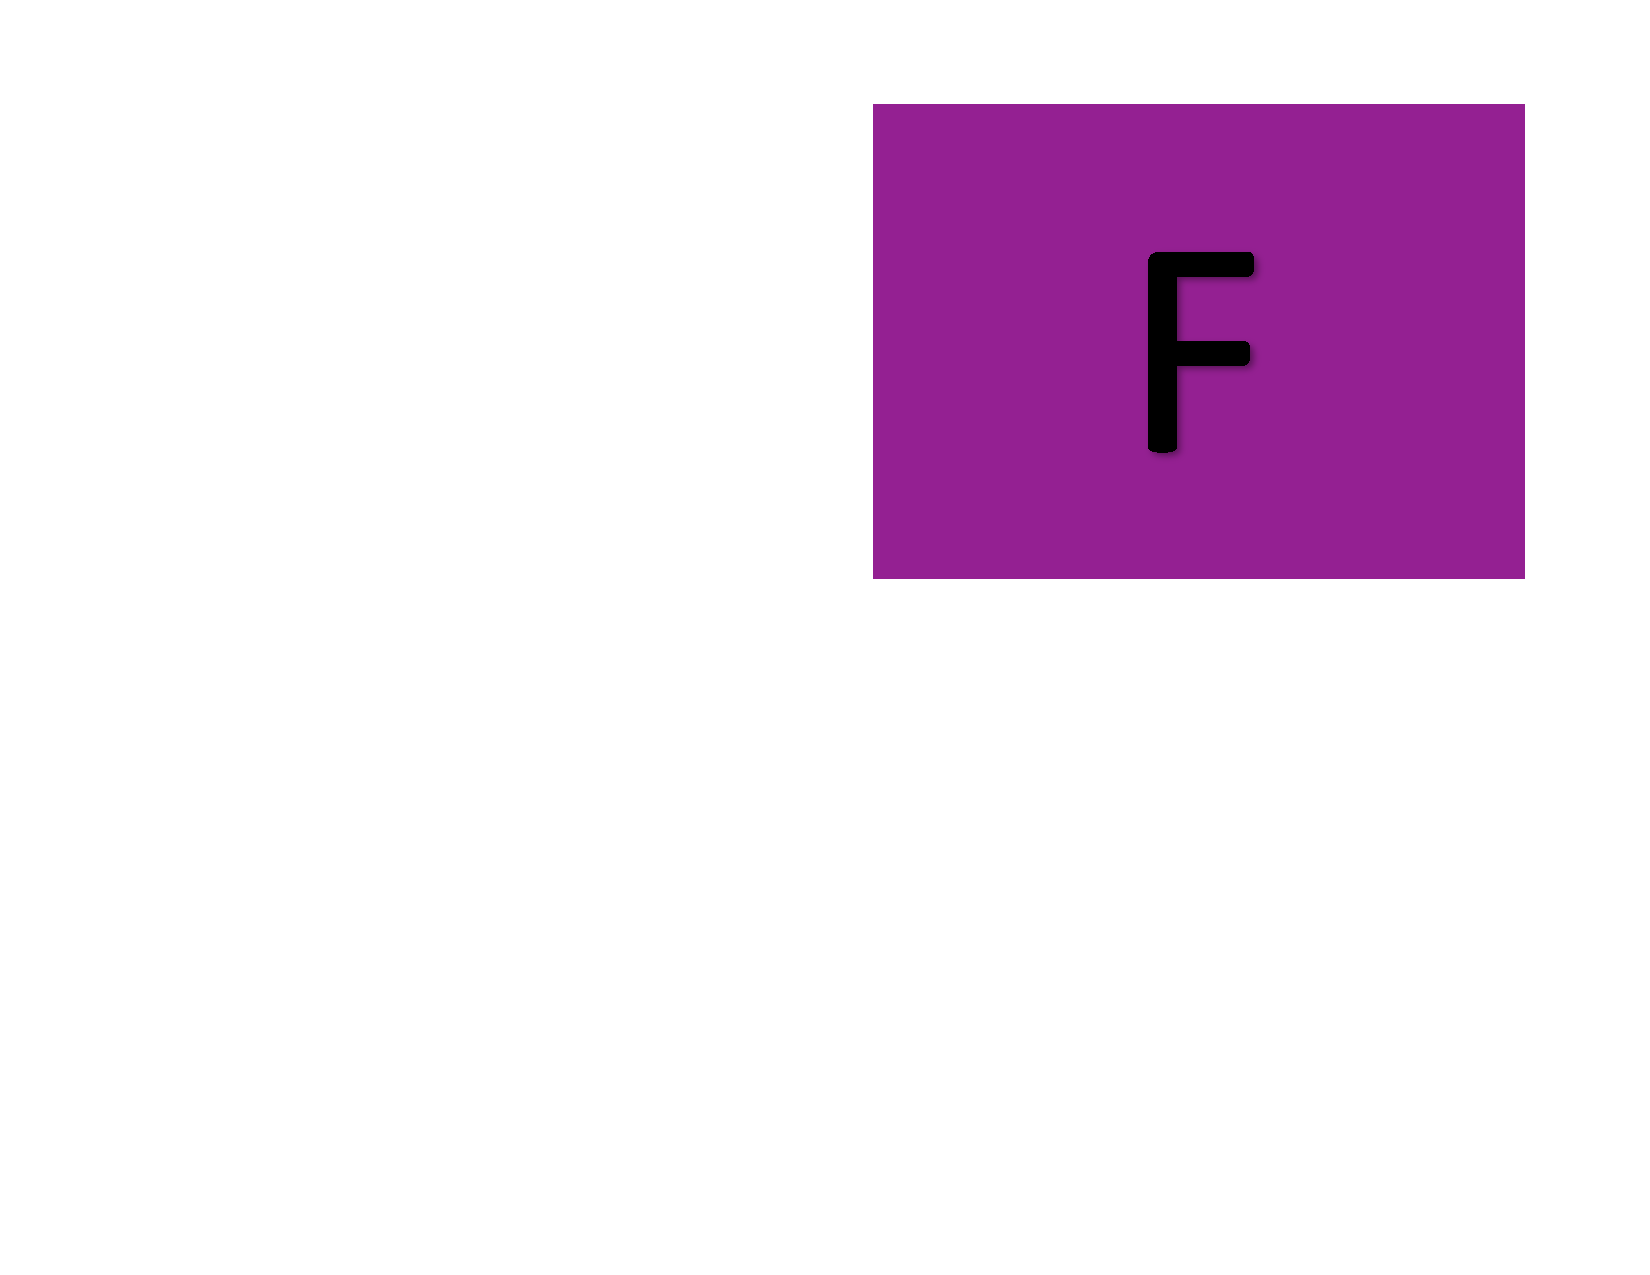
\includegraphics[width=0.8cm,height=0.5cm]{../../Lectures/figures/F}} ]  }


\newcommand{\hide}[1]{\underline{\phantom{#1 #1}}}

\usepackage{setspace}

\onehalfspacing

\begin{document}
	
	
	\lecture{8: Amortized Analysis}{February 11, 2025}
	
	\paragraph{Course Logistics}
	
	\begin{itemize}
		\item Amortized analysis: Chapter 17
		\item First test is Thursday
	\end{itemize}
	

\section{Representing numbers in binary}
We represent a number $x \in \mathbb{N}$ in binary by a vector of bits $A[0..k]$, where $A[i] \in \{0,1\}$ and
\begin{equation*}
	x = \sum_{i = 0}^k  A[i] \cdot 2^i
\end{equation*}

%	\paragraph{Examples}


\pagebreak 

\section{The Binary Counter Problem}
Let \textsc{Increment} be an algorithm that takes in a binary vector and adds one to the binary number that it represents.
\begin{algorithm}
	\textsc{Increment}($A$)
	\begin{algorithmic}
		\State $i = 0$
		\While{$i < A.length$ and $A[i] == 1$}
		\State $A[i] = 0$
		\State $i = i+1$
		\EndWhile
		\If{$i < A.length$}
		\State
		\State \hide{$A[i] = 1$}
		\State
		\EndIf
	\end{algorithmic}
\end{algorithm}

\vfill

\QU
If $A$ is length $k$ binary vector, what is the worst-case runtime for calling $\textsc{Increment}(A)$?
\begin{itemize}
	\aitem $O(1)$
	\bitem $O(\log k)$
	\citem $O(k)$
	\ditem $O(n)$
\end{itemize}
\end{Qu}

\pagebreak
\subsection{The actual cost of each iteration}
Assume it takes $O(1)$ time to check an entry of $A$ or to flip its bit. At each step, the runtime is then just $O(\text{number of flipped bits})$, so we will say the cost of an iteration is 
\begin{center}
$c_i$ = \hide{number of flipped bits in iteration $i$.}
\end{center}

\emph{Key idea:} Separate the costs that happen \hide{at each entry $A[j]$}\\ \\

\vs{1cm} 

{\Huge
\begin{tabular}{ l || p{1cm} | p{1cm} | p{1cm} | p{1cm} | p{1cm} |}
	\hline
	0& 	0 & 0 & 0 & 0 & 0\\
	\hline 
	1& 	0 & 0 & 0 & 0 & 1\\
	\hline 
	2& 	0 & 0 & 0 & 1 & 0\\
	\hline 
	3& 	0 & 0 & 0 & 1 & 1\\
	\hline 
	4& 	0 & 0 & 1 & 0 & 0\\
	\hline 
	5& 	0 & 0 & 1 & 0 & 1\\
	\hline 
	6& 	0 & 0 & 1 & 1 & 0\\
	\hline 
	7& 	0 & 0 & 1 & 1 & 1\\
	\hline 
	8& 	0 & 1 & 0 & 0 & 0\\
	\hline 
	9& 	0 & 1 & 0 & 0 & 1\\
	\hline 
	10& 	0 & 1 & 0 & 1 & 0\\
	\hline 
	11& 	0 & 1 & 0 & 1 & 1\\
	\hline 
\end{tabular}
}

\newpage 

\subsection{Technique 1: Aggregate Analysis}
Let $T(n)$ be the total number of number of flipped bits in $n$ increments.

\QU
Look at the table on the last page, and observe how often the bit in position $A[j]$ is flipping. If you wish, fill in the number of total flipped bits at each increment. What is the total cost of calling \textsc{Increment} $n$ times?
\begin{itemize}
\aitem $O(n)$
\bitem $O(k)$
\citem $O(nk)$ 
\ditem $O(n^2)$
\end{itemize}
\end{Qu}


\pagebreak
\subsection{Technique 2: The accounting method}
\begin{itemize}
\item $c_i = $ the actual number of bits flipped
\item $\hat{c}_i$ amortized cost for flipping bits: \hide{\$2 for setting 0 to 1}
\end{itemize}
{\Huge
\begin{tabular}{ l || p{1cm} | p{1cm} | p{1cm} | p{1cm} | p{1cm} |}
\hline
0& 	0 & 0 & 0 & 0 & 0\\
\hline 
1& 	0 & 0 & 0 & 0 & 1\\
\hline 
2& 	0 & 0 & 0 & 1 & 0\\
\hline 
3& 	0 & 0 & 0 & 1 & 1\\
\hline 
4& 	0 & 0 & 1 & 0 & 0\\
\hline 
5& 	0 & 0 & 1 & 0 & 1\\
\hline 
6& 	0 & 0 & 1 & 1 & 0\\
\hline 
7& 	0 & 0 & 1 & 1 & 1\\
\hline 
8& 	0 & 1 & 0 & 0 & 0\\
\hline 
9& 	0 & 1 & 0 & 0 & 1\\
\hline 
\end{tabular}
}
\begin{algorithm}
\textsc{Increment}($A$)
\begin{algorithmic}
\State $i = 0$
\While{$i < A.length$ and $A[i] == 1$}
\State $A[i] = 0$
\State $i = i+1$
\EndWhile
\If{$i < A.length$}
\State $A[i] = 1$
\EndIf
\end{algorithmic}
\end{algorithm}

\pagebreak
\subsection{Technique 3: The potential method}

\textbf{Step 0:} Identify data structure, potential function, and costs.
\begin{itemize}
\item $c_i$: the actual number of flipped bits at iteration $i$
\item data structure: \hide{the counter $A$}, with state $D_i$ after iteration $i$
\item $\Phi(D_i) = b_i$ = \hide{number of 1's in the counter} % after iteration $i$
\item $\hat{c}_i = $ \hide{is the amortized cost}
\end{itemize}

\textbf{Step 1: Check that $\Phi(D_i) \geq \Phi(D_0)$}

\vspace{3cm}

\textbf{Step 2: Compute and bound amortized costs}\\

Let $t_i$ be the number of bits that are set to $0$ (\emph{while} loop in algorithm) in iteration $i$.\\

If $b_i = 0$, this means we had $A = [1 \; 1 \; 1 \; \cdots \; 1]$ in iteration $i$, and incrementing turned it into $A = [0 \; 0 \; 0 \; \cdots \; 0]$, meaning $b_{i-1} = t_i = k$. \\

\begin{Qu}
If $b_i > 0$, which of these is the right expression for $b_i$?
\begin{itemize}
\aitem $b_i = b_{i-1} + 1$
\bitem $b_i = t_i + 1$
\citem $b_i = b_{i-1} + t_i$ 
\ditem $b_i = b_{i-1} - t_i$ 
\eitem $b_i = b_{i-1} + t_i + 1$
\fitem $b_i = b_{i-1} - t_i + 1$
\end{itemize}
\end{Qu}

\pagebreak
Whether or not $b_i = 0$, we have a bound of \hide{$b_i \leq b_{i-1} - t_i  + 1$.}\\

We can then compute the amortized cost and overall runtime bound:


%\pagebreak
%\subsection{Binary counter problem: potential method}
%
%\textbf{Step 0:} Identify data structure, potential function, and costs.
%\begin{itemize}
%	\item $c_i$: the actual number of flipped bits at iteration $i$
%	\item data structure: the counter $A$, with state $D_i$ after iteration $i$
%	\item $\Phi(D_i) = b_i$ = number of 1's in the counter after iteration $i$
%	\item $\hat{c}_i = c_i + \Phi(D_i) - \Phi(D_{i-1})$ is the amortized cost
%\end{itemize}
%
%\textbf{Step 1: Check that $\Phi(D_i) \geq \Phi(D_0)$}
%
%At step zero we know $\Phi(D_0) = 0$, since there are no 1's in the binary representation of 0. \\
%
%At step $i$, we still have $\Phi(D_i) \geq 0$, since we can't have a negative number of zeros. \\
%
%
%\textbf{Step 2: Compute and bound amortized costs}\\
%
%Let $t_i$ be the number of bits that are set to $0$ (\emph{while} loop in algorithm) in iteration $i$.\\
%
%If $b_i = 0$, this means we had $A = [1 \; 1 \; 1 \; \cdots \; 1]$ in iteration $i$, and incrementing turned it into $A = [0 \; 0 \; 0 \; \cdots \; 0]$, meaning $b_{i-1} = t_i = k$. \\
%
%\begin{Qu}
%	If $b_i > 0$, which of these is the right expression for $b_i$?
%	\begin{itemize}
%		\aitem $b_i = b_{i-1} + 1$
%		\bitem $b_i = b_{i-1} + t_i + 1$
%		\citem $b_i = b_{i-1} - t_i + 1$
%		\ditem $b_i = b_{i-1} + t_i$ 
%		\eitem $b_i = b_{i-1} - t_i$ 
%		\fitem $b_i = t_i + 1$
%	\end{itemize}
%\end{Qu}
%
%\pagebreak
%Whether or not $b_i = 0$, we have a bound of \hide{$b_i \leq b_{i-1} - t_i  + 1$.}\\
%
%We can then compute the amortized cost and overall runtime bound:
%
%
%
%\pagebreak
%\textbf{What happens if we do not start with an empty counter?} 
%
%\vs{1cm}
%
%This means that \hide{$\Phi(D_0) = b_0 \geq 1$.}
%



\end{document}
